\documentclass{article}
\usepackage{graphicx}
\usepackage[margin=1in]{geometry}
\usepackage{tikz} % for diagram
\usetikzlibrary{positioning}

\title{\bf{Project Proposal:\\Real Estate Development Classifier}}
% \author{Monem Moheq}
\date{June 2026}

\begin{document}

\maketitle

\section*{Group Information}
Group Name: Heron Pond\\ % Unoficial, change if you want
Group Number: 14
\\Members:
% list yourselves here
% also add your sfu student number 
\begin{itemize}
    \item Monem Moheq, mma323@sfu.ca, 301591088
    \item Finley Thomson, fgt@sfu.ca, 301591261
    \item Srinivas Suggu, ssuggu@sfu.ca, 301408443
    \item Jarrod Hwang, sha293@sfu.ca, 301541546
\end{itemize}

% Describe what your AI system will do:
% What problem is it solving?
% What kind of input will it take, and what will it output?
% What AI techniques do you plan to use? (e.g., supervised learning, classification, search, planning, etc.)
% Include a simple system diagram if possible
\section*{Project Idea}
Evaluating potential real estate development opportunities is a task that can be streamlined with an AI model. Such a model would allow for a quick, simple analysis of a large number of such opportunities, allowing time and effort to be spent on those which are likely to be fruitful, without having to sift through the many that are not. We aim to develop a model that takes in various economic and qualitative factors such as location, pricing, size, income level, nearby amenities, etc., to deliver an investment potential rating. More specifically, it classifies the property as having a high, medium, or low return on investment (ROI). The key driver of the model will be ordinal logistic regression and a random forest classifier that will vote in order to determine an investments potential ROI classification. 

\begin{center}
    
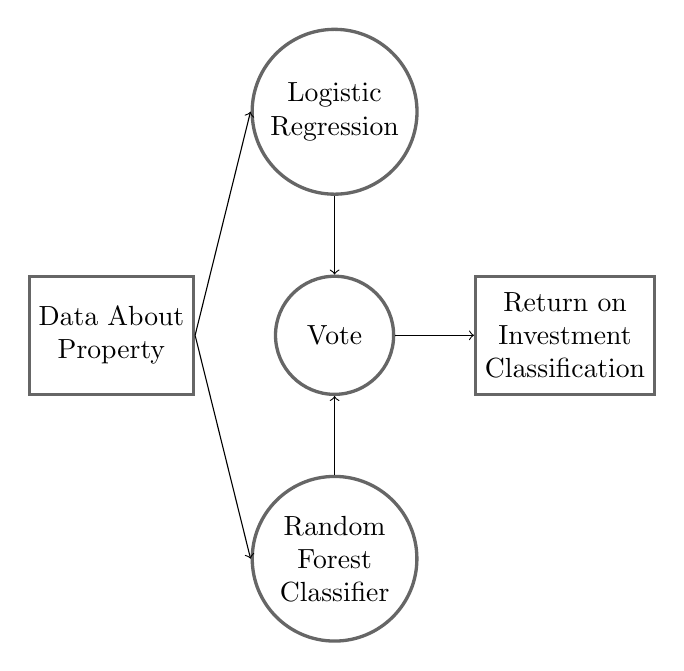
\begin{tikzpicture}[
roundnode/.style={circle, draw=black!60, fill=white!5, very thick, minimum size=15mm},
squarednode/.style={rectangle, draw=black!60, fill=white!5, very thick, minimum size=15mm},
]

\node[roundnode, align=center]        (Vote)                         {Vote};
\node[roundnode, align=center]        (Logreg)       [above=of Vote] {Logistic\\Regression};
\node[squarednode, align=center]      (Output)       [right=of Vote] {Return on\\ Investment\\ Classification}; 
\node[squarednode, align=center]      (Input)        [left=of Vote] {Data About\\ Property};
\node[roundnode, align=center]        (Forest)       [below=of Vote] {Random\\ Forest\\ Classifier}; 

\draw[->] (Input.east) -- (Forest.west);
\draw[->] (Input.east) -- (Logreg.west);
\draw[->] (Logreg.south) -- (Vote.north);
\draw[->] (Forest.north) -- (Vote.south);
\draw[->] (Vote.east) -- (Output.west);

\end{tikzpicture}

\end{center}

% Tools and Resources
% Any external tools/libraries needed (e.g., scikit-learn, PyTorch, OpenCV)
% Any data you'll use (e.g., UCI dataset, synthetic images, simulation data)
% Will you generate your own dataset?
% Will you use a simulator (e.g., PyBullet, OpenAI Gym) or work with real-world data?
%\section*{Tools and Resources}
%Ordinal logistic regression is supported by the statsmodels library in python. The data we will use to create this classifier will be current and historic pricing data from official Multiple Listing Service (MLS) listings, current urban development statistics compiled from the Canadian Mortgage and Housing Corporation (CMHC) survey data, and demographics data gathered from Statistics Canada. Both training and testing data will be real world as we can then test the model against historical development sites comparing how they performed to how the model assesses the investment potential. 

\section*{Tools and Resources}
The system will be implemented primarily in Python. We will use \texttt{pandas} and \texttt{NumPy} for data cleaning, merging, and feature engineering, and \texttt{scikit-learn} for preprocessing tasks such as train-test splitting, scaling numerical features, and evaluating model performance. The main model will use ordinal logistic regression, which is supported by the \texttt{statsmodels} library and a random forest classifier, supported by the \texttt{scikit-learn} library. 

% I moved this line to the Milestione 2 section as I agree this would be a good goal to aim for if time permits. If time permits, we may also use \texttt{PyTorch} to experiment with a simple neural-network-based classifier and compare its performance against the ordinal logistic regression baseline.

The data we will use to create this classifier will include current and historical pricing data from official Multiple Listing Service (MLS) listings as well as property evaluations from BC Assessment, current urban development statistics compiled from Canada Mortgage and Housing Corporation (CMHC) survey data, and demographics data gathered from Statistics Canada. Both training and testing data will be real-world data rather than simulated data. This will allow us to test the model against historical development sites by comparing how those sites actually performed to how the model assesses their investment risk. If complete MLS data is difficult to access, we will limit the minimal viable system to a smaller localized dataset or use publicly available property and neighbourhood-level data for early testing.

\section*{Project Timeline}

\subsection*{Milestone 1: July 1\textsuperscript{st}}

By July 1\textsuperscript{st}, we will aim to have compiled a large amount of data for training, as well as to have an agent that is able to receive a basic set of data about a given property and output a classification, regardless of how precisely correct it is. In essence, we hope to have a rudimentary form of the classifier trained such that we can input data and receive reasonable result as compared to historical data.

\subsection*{Milestone 2: July 29\textsuperscript{th}}

By this point, we hope to have a much more fine-tuned model, able to take in more data points about a property in order to provide a more precise result and, overall, deliver more accurate assessment of investment risk. If time permits, we may also use \texttt{PyTorch} to experiment with a simple neural-network-based classifier and compare its performance against the ordinal logistic regression baseline.

% Minimal Viable System
% Briefly describe:
% What is the simplest working version of your system?
% What is the core functionality you’ll prioritize first?
% How could your system be useful or insightful even in a basic form?
\section*{Minimal Viable System}

\noindent \textbf{Simplest Working Version: }
The simplest working version is a baseline ordinal logistic regression model and a random forest classifier trained on a localized subset of features, such as past price trends, property size, and average neighbourhood income. It will take these basic inputs and classify properties into High, Medium, or Low ROI without requiring complex spatial data processing.

\vspace{0.5cm}

\noindent \textbf{Core Functionality: }
We will prioritize establishing a clean data pipeline to merge historical MLS pricing data with Statistics Canada demographic data. Once merged, we will mathematically label the historical outcomes and successfully execute a basic train-test split using the \texttt{statsmodels} and \texttt{scikit-learn} libraries to ensure the classification logic functions correctly.

\vspace{0.5cm}
\noindent \textbf{How it is useful in a basic form: }
Even this basic system will serve as a preliminary screening tool to rapidly filter out low-potential properties, allowing developers to focus their manual analysis on higher-yield opportunities. Additionally, analyzing the model's regression coefficients will provide immediate insight into which baseline economic factors have the strongest predictive power for investment risk.

\end{document}

